% https://tex.stackexchange.com/questions/458152/hidden-pages-in-latex
\optional{
%\Hide
% https://tex.stackexchange.com/questions/228729/how-to-hide-chapter-numbering-in-table-of-contents
\chapter*{\emph{Sashimi}: A toolkit for facilitating high-throughput organismal image segmentation using deep learning}
\addcontentsline{toc}{chapter}{\emph{Sashimi}: A toolkit for facilitating high-throughput organismal image segmentation using deep learning}
}

\clearpage

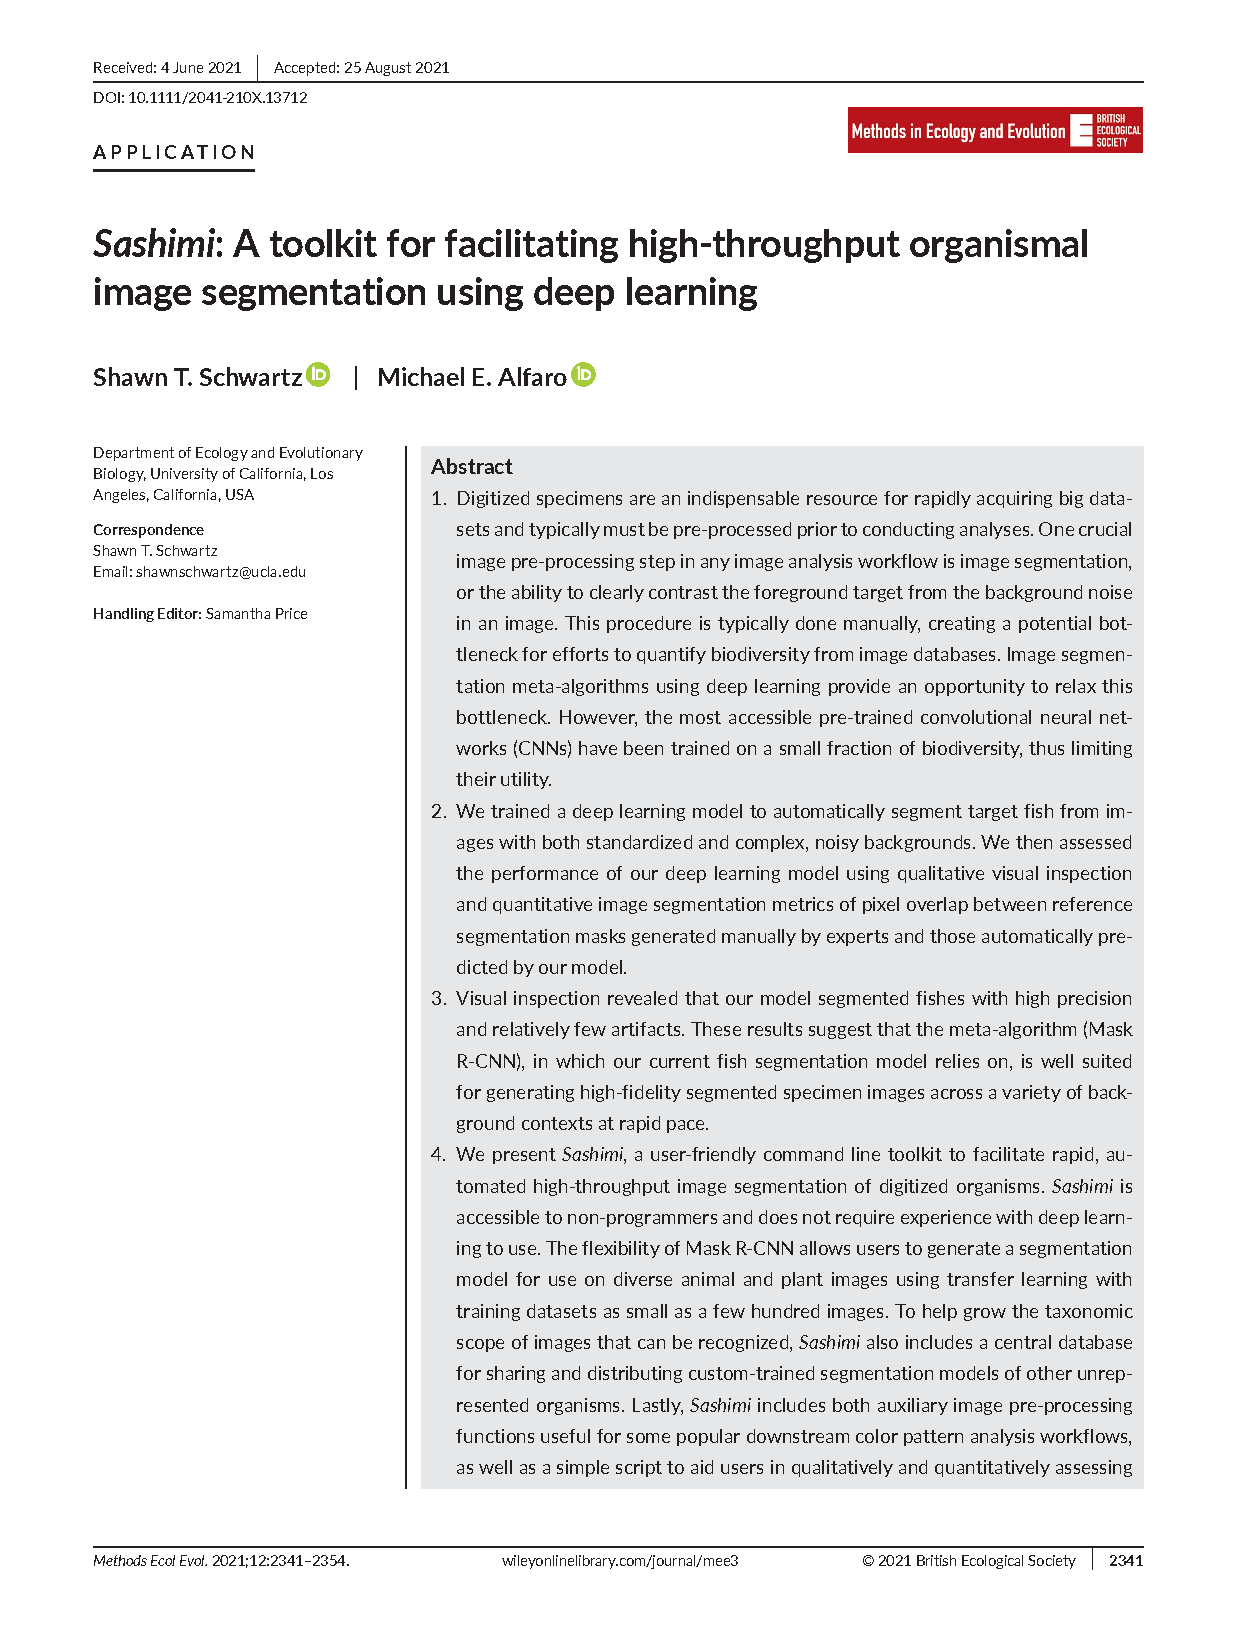
\includepdf[scale=0.85, pages=1-14, pagecommand={}, addtotoc={
     1,section,1,Abstract,abstract,
     2,section,1,Introduction,intro,
     4,section,1,Materials and Methods,materialsandmethod,
     4,subsection,1,Mask R-CNN architecture,architecture,
     4,subsection,1,Model training dataset acquisition,dataset,
     4,subsection,1,Model training procedure,training,
     4,subsection,1,Automated segmentation pipeline,pipeline,
     4,subsection,1,\emph{Sashimi} online model repository,repo,
     4,subsection,1,Evaluating fish segmentation model efficacy,modeleval,
     4,subsubsection,2,Qualitative image segmentation evaluation,qualseg,
     5,subsubsection,2,Quantitative image segmentation evaluation metrics,quantseg,
     7,subsection,1,Statistics,stats,
     7,section,1,Results,results,
     7,subsection,1,Qualitative image segmentation evaluation,qualsegres,
     8,subsection,1,Quantitative image segmentation evaluation metrics,quantsegres,
     9,section,1,Discussion,discussion,
     11,section,1,Acknowledgements,acks,
     11,section,1,Conflict of Interest,interest,
     11,section,1,Authors' Contributions,contrib,
     12,section,1,Peer Review,peerrev,
     12,section,1,Data Availability Statement,openscience,
     12,section,1,ORCID,orcid,
     12,section,1,References,refs
     }, addtolist={5,figure,Examples of diverse fish images used for model training,fig1,
     6,figure,Examples of predicted segmentation masks generated by custom-trained fish segmentation model,fig2,
     7,figure,Examples of fish images automatically segmented by \emph{Sashimi},fig3,
     8,figure,Butterflyfishes segmented by humans along with naïve and custom-trained COCO models,fig4,
     9,figure,(a) \emph{Forcipiger} Butterflyfishes segmented by humans and \emph{Sashimi}; (b) Automatically segmented fishes with stray pixels,fig5,
     10,figure,Segmentation of novel fish images in natural noisy contexts,fig6,
     11,figure,Image segmentation evaluation metrics,fig7,
     11,table,Post hoc comparisons for the main effect of evaluation metric,tab1
     }]{pdfs/mee_main.pdf}
    %  \startsupplement
    
    % https://tex.stackexchange.com/questions/104479/table-numbering-style/104484
    % https://tex.stackexchange.com/questions/85776/change-figure-numbering-for-appendix
    \appendix
    \counterwithin{table}{section}
    \renewcommand{\thesection}{S\arabic{section}}
    \renewcommand{\thetable}{S\arabic{table}}
\includepdf[scale=1, pages=1-78, pagecommand={}, addtotoc={
1,section,1,Supporting Information,suppinfo,
4,subsection,1,Quantitative image segmentation evaluation metrics for novel test set,quantimgevalnovel,
8,subsection,1,Color pattern analysis comparison,colorpatternanalysis,
10,subsection,1,Results,suppres,
14,subsection,1,iNaturalist novel test set (\textit{n} = 30) visual evaluations,inatvizeval,
45,subsection,1,J.E. Randall novel test set (\textit{n} = 30) visual evaluations,randallvizeval,
76,subsection,1,References,supprefs}, addtolist={1,table,Post hoc comparisons for the interaction between accuracy metric and image source (validation set),s1,
5,table,Post hoc comparisons for the main effect of evaluation metric (test set),s2,
6,table,Post hoc comparisons for the interaction between accuracy metric and image source (test set),s3,
11,table,MANOVA,s4,
13,table,Descriptive statistics for color pattern geometry variables,s5}]{pdfs/mee_supp.pdf}